\documentclass[10pt,aspectratio=43]{beamer}

\usepackage{graphicx}
\graphicspath{{../internship_report/prebuilt_images/}{../internship_beamer/gif/}}
\usepackage[rotationcw % clockwise, default is counterclockwise
			]{beamerthemeGlobalUniNA}

\usepackage[utf8]{inputenc}
\usepackage[english]{babel}
\usepackage[T1]{fontenc}
\usepackage{csquotes}
\usepackage{copyrightbox}
\usepackage{cleveref}
\usepackage{hyperref}
\usepackage[scaled]{beramono}
\usepackage[scale=1.05]{AlegreyaSans}
\usepackage{sty_tl}
\usepackage{subcaption}
\usepackage{minted}
\pgfplotsset{compat=1.17}
\usetikzlibrary{spy}
\usepackage[round]{natbib}
\bibliographystyle{plainnat}

%%%%%%%%%%%%%%%%%%%%%%%%%%%%%%%%%%%%%%%%%%%%%%%%%%%%%%%%%%%%%%%%%%%%%%%%%%%%%%%
% footnote setting: (1), (2), etc.
\usepackage{fnpct}

% Configure style for custom doubled line
\newcommand*{\doublerule}{\hrule width \hsize height 1pt \kern 0.5mm \hrule width \hsize height 2pt}

% Configure function to fill line with doubled line
\newcommand\doublerulefill{\leavevmode\leaders\vbox{\hrule width .1pt\kern1pt\hrule}\hfill\kern0pt }


\newcommand{\mytheorem}[2]{
    \doublerulefill\ \framebox{\textbf{#1}}\ \doublerulefill
    \vspace{0.1cm}
    #2
    \doublerulefill
}

\definecolor{javared}{rgb}{0.6,0,0} % for strings
\definecolor{javagreen}{rgb}{0.25,0.5,0.35} % comments
\definecolor{javapurple}{rgb}{0.5,0,0.35} % keywords
\definecolor{javadocblue}{rgb}{0.25,0.35,0.75} % javadoc
\definecolor{marron}{rgb}{0.64,0.16,0.16}
\definecolor{orange_js}{RGB}{230,159,0}

\newcommand{\mybold}[1]{\textcolor{marron}{\textbf{#1}}}
\newcommand{\cRm}[1]{\textsc{\romannumeral #1}}

\usepackage{csquotes}
\usepackage{amsmath,amsfonts,amsthm,amssymb}

%%%%%%%%%%%%%%%%%%%%%%%%%%%%%%%%%%%%%%%%%%%%%%%%%%%%%%%%%%%%%%%%%%%%%%%%%%%%%%%
%%%%%%%%%%%%%%%%%%%%%%%%%%%%%%%%%%%%%%%%%%%%%%%%%%%%%%%%%%%%%%%%%%%%%%%%%%%%%%%
% HEADER
%%%%%%%%%%%%%%%%%%%%%%%%%%%%%%%%%%%%%%%%%%%%%%%%%%%%%%%%%%%%%%%%%%%%%%%%%%%%%%%
%%%%%%%%%%%%%%%%%%%%%%%%%%%%%%%%%%%%%%%%%%%%%%%%%%%%%%%%%%%%%%%%%%%%%%%%%%%%%%%

\title[] %shown at the top of frames
{High dimensional penalized linear models with interactions using graphics card
} %shown in title frame
\subtitle{Internship supervised by Joseph Salmon and Benjamin Charlier}

\date{07-2021} % explicitly set date instead of \today

\author[]%shown at the top of frames
{%shown in title frame
	{Lefort Tanguy}%
}

\institute[
]
{% is placed on the bottom of the title page
    University of Montpellier
}

\titlegraphic{% logos are put at the bottom-right part of the page
    \includegraphics[width=3cm]{Logo}\hspace{1cm} % also support multi-logos
    \includegraphics[width=3cm]{imag_logo}~ % up to 3 (after it gets messy)
    %\includegraphics[width=2cm]{Logo.pdf} % if more, combine them in one image.
}

\setbeamercolor{itemize subitem}{fg=javadocblue}
\setbeamertemplate{itemize subitem}[triangle]

%%%%%%%%%%%%%%%%%%%%%%%%%%%%%%%%%%%%%%%%%%%%%%%%%%%%%%%%%%%%%%%%%%%%%%%%%%%%%%%
%%%%%%%%%%%%%%%%%%%%%%%%       PLAN      %%%%%%%%%%%%%%%%%%%%%%%%%%%%%%%%%%%%%%
%%%%%%%%%%%%%%%%%%%%%%%%%%%%%%%%%%%%%%%%%%%%%%%%%%%%%%%%%%%%%%%%%%%%%%%%%%%%%%%

\begin{document}
\maketitle


%%%%%%%%%%%%%%%%%%%%%%%%%%%
% Table of contents
%%%%%%%%%%%%%%%%%%%%%%%%%%%
\begin{frame}{Content}{}
    \tableofcontents
\end{frame}

\section{Introduction}

%%%%%%%%%%%%%%%%%%%%%%
% Introduction
%%%%%%%%%%%%%%%%%%%%%%
\subsection{Linear model with penalties}
\begin{frame}{Introduction}{The Linear Model}
We denote $X \in \bbR^{n \times p}, y \in \bbR^n$ and
$\beta \in \bbR^p$ such that $y\simeq X\beta$. \\
Ordinary least squares:
\[\hat\beta^{ls} = \argmin_{\beta} \frac{1}{2n}\|y-X\beta\|_2^2
\Longleftrightarrow \hat \beta = (X^\top X)^{-1}X^\top y \enspace.\]

Problems with high dimensions:
\begin{itemize}
\item if $p>n$ we lose the uniqueness,
\begin{onlyenv}<2>
    \begin{itemize}
        \item  \color{red}{make the problem strictly convex.}
    \end{itemize}
\end{onlyenv}
\item $X^\top X$ may be ill conditioned
($\kappa = \frac{\text{largest singular value}}{
    \text{smallest singular value}} \gg $ )
    because of multicolinearity amongst features,
\begin{onlyenv}<2->
    \begin{itemize}
        \item \color{red}{Shift spectrum by a small quantity using
        $\ell_2$ penalty.}
    \end{itemize}
\end{onlyenv}
\item too many active features is not interpretable (genomics dataset),
\begin{onlyenv}<2->
    \begin{itemize}
        \item \color{red}{Feature selection using $\ell_1$ penalty.}
    \end{itemize}
\end{onlyenv}\end{itemize}
\end{frame}

\subsection{Elastic-Net with interactions}
\begin{frame}{Introduction}{Elastic-Net estimator \citep{Zou_Hastie05}}
Combination of LASSO \citep{Tibshirani96} and
Ridge\citep{Tikhonov43}:
\begin{block}{Elastic-Net}
Considering $\lambda_1,\lambda_2>0$ penalties,
\begin{align*}
    \hat\beta^{enet} \in \argmin_{\beta \in \bbR^p}\frac{1}{2n}\norm{y - X\beta}_2^2
    + \lambda_1 \norm{\beta}_1
    + \frac{\lambda_2}{2} \norm{\beta}_2^2 \enspace.
\end{align*}
\end{block}
\begin{onlyenv}<2>
    And if we add the first order interactions to the model:
    \begin{block}{Elastic-Net with interactions}
    The interactions matrix is $Z\in\bbR^{n\times q}$, $q=\tfrac{p(p+1)}{2}$
     and coefficients are $\Theta\in\bbR^q$.
        \begin{align*}
        \hat\beta^{\textcolor{red}{inter}}
        \in \argmin_{\substack{\beta \in \bbR^p \\ \Theta \in \bbR^q}}
        \frac{1}{2n}\norm{y - X\beta - Z\Theta}_2^2
        & + \lambda_{\beta,\ell_1} \norm{\beta}_1
        + \frac{\lambda_{\beta, \ell_2}}{2} \norm{\beta}_2^2 \\
        & \textcolor{red}{+ \lambda_{\Theta,\ell_1} \norm{\Theta}_1
        + \frac{\lambda_{\Theta, \ell_2}}{2} \norm{\Theta}_2^2}
        \enspace.
    \end{align*}
\end{block}
\end{onlyenv}
\end{frame}

\begin{frame}{Optimization problem}
\textbf{Our goal:} Solve the Elastic-Net problem
\begin{itemize}
    \item for high dimensional genomics data,
    \item using graphics card parallelization,
    \item at least as fast as currently used algorithms like Coordinate Descent
    with interactions \citep{Bascou_Lebre_Salmon20}.
\end{itemize}

\begin{onlyenv}<2>
\textbf{Problems:}
    \begin{itemize}
        \item the interactions matrix is not storable in high dimensions,
        \item graphics cards need a lot of data to parallelize operations
        efficiently,
        \item we use solvers, but when do we stop them ?
    \end{itemize}
\end{onlyenv}
\end{frame}

\section{Gradient Descent solvers}
\begin{frame}{From gradient to coordinate descent
    }{On least squares problem}
Minimize $F(\beta)=\frac{1}{2n}\norm{y - X\beta}_2^2$:
with step $\eta>0$ at epoch $k\in\bbN$,
\begin{block}{Gradient Descent: 1 problem of dimension p}
\[\beta^{k+1} \longleftarrow \beta^k - \eta \LaTeXunderbrace{\frac{1}{n}X^\top (X\beta^k - y)}_{
    \frac{\partial F}{\partial \beta}(\beta^k)
}\enspace.\]
\end{block}
\begin{onlyenv}<2>
\begin{block}{Coordinate Descent: p problems of dimension 1}
For $j=1,\dots,p$,
\[\beta^{k+1}_j \longleftarrow \beta^k_j - \eta \LaTeXunderbrace{\frac{1}{n}x_j^\top (X\beta^k - y)}_{
    \frac{\partial F}{\partial \beta_j}(\beta^k)
}\enspace.\]
\end{block}
\end{onlyenv}
\end{frame}

\begin{frame}{Visualization of the behavior}
\foreach \index in {1, ..., 12}{
    \begin{onlyenv}<\index>
        \begin{figure}
        \centering
        \includegraphics[width=.8\textwidth, clip,
        trim={0cm 0cm 0cm 1.5cm}]{temp\index.pdf}\par%
        \end{figure}
    \end{onlyenv}
}
\end{frame}

\subsection{Proximal operator}
\begin{frame}{And with a non differentiable function?}{Proximal operators}
\[\argmin_{\beta\in \bbR^p}
\LaTeXunderbrace{\frac{1}{2n}\norm{y-X\beta}_2^2}_{\text{smooth } F(\beta)} +
\LaTeXunderbrace{
    \lambda_1 \norm{\beta}_1 + \frac{\lambda_2}{2}\norm{\beta}_2^2}_{
\text{non-smooth separable } g(\beta)
}\]
\begin{onlyenv}<2>
Gradient descent on $F$:
\[\beta^{k+1} \longleftarrow \beta^k - \eta \frac{1}{n}X^\top(X\beta - y)\]
\end{onlyenv}

\begin{onlyenv}<3>
\textcolor{red}{Proximal} Gradient descent on $F+g$:
\[\beta^{k+1} \longleftarrow
\textcolor{red}{\prox_{\eta g}\big( }\beta^k -
 \eta \frac{1}{n}X^\top(X\beta - y)\textcolor{red}{\big)}\enspace.\]

\begin{block}{Proximal operator}
Let $f$ a convex proper closed function, for $\mu>0$:
\begin{align*}
\prox_{\mu f}(u) = \argmin_{x\in\dom f}\left\{
    f(x) + \frac{1}{2\mu}\norm{x-u}_2^2
\right\} \enspace.
\end{align*}
\end{block}
\end{onlyenv}

\end{frame}


\subsection{Accelerations}
\begin{frame}{Accelerate the algorithms}
Possibilities to use accelerations:
\begin{itemize}
    \setlength\itemsep{1em}
    \item Theoretical:
    \begin{itemize}
        \item inertial: heavy ball-like \citep{nesterov27method},
        \item structure of the iterates: \citep{bertrand2021anderson},
        \item stochastic directions: \citep{nesterov2012efficiency}.
    \end{itemize}
    \item Computational:
    \begin{itemize}
        \item \texttt{Numba} library: \citep{lam2015numba},
        \item GPU acceleration with \texttt{CUDA}.
    \end{itemize}
\end{itemize}
\end{frame}



\subsection{First order interactions}
\begin{frame}{Building the interactions}{First order interactions by block}
See the interactions as blocks generated from $X=[x_1|\dots|x_p]$:
\begin{figure}[h]
    \centering
    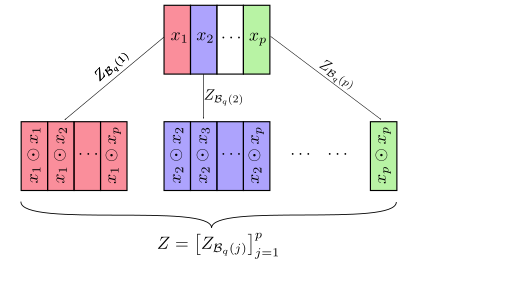
\includegraphics[width=.9\textwidth]{building_interactions.pdf}
\end{figure}
\end{frame}



\begin{frame}{Conclusion}
    dfghhgfdsdfgfd
\end{frame}


%%%%%%%%%%%%%%%%%
% Biblio
%%%%%%%%%%%%%%%%%

\begin{frame}[allowframebreaks]{}
    \frametitle{References}
    \bibliography{../internship_report/sty/biblio.bib}
\end{frame}

\end{document}
